\documentclass[10pt,pscyr,nonums]{hedlab}
\usepackage[russian]{babel}
\usepackage{hedmaths}
\usepackage{graphicx}
\graphicspath{{images/}, {plots/}}

\newgeometry{top=1.5cm, bottom=1.5cm, left=1cm, right=1cm}

\student{Чечеткин И. А., Ф-469}
\date{16.10.2013}
\labnum{605}
\labname{Определение ширины запрещенной зоны в кристалле диэлектрика}

\begin{document}
  \makeheader

  \emph{Цель работы:} изучение закономерностей поглощения света кристаллами с
  точки зрения зонной теории. Определение границы основного поглощения и
  ширины запрещенной зоны кристалла титаната бария.
  
  \emph{Используемые при расчетах формулы:}
  \( \tau = (J - J_T)/(J_0 - J_T); \ \Delta E = hc/\lambda_0 \).

  \begin{figure}[h!]
    \center
    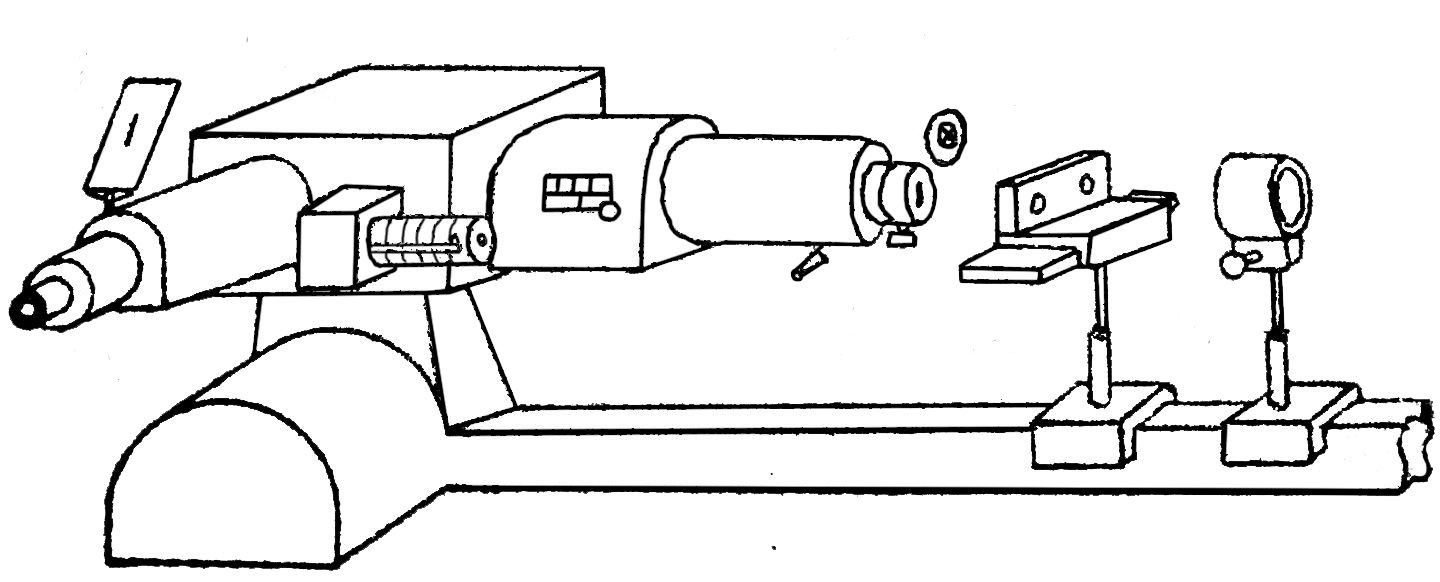
\includegraphics[width=.5\textwidth]{appearance} \\
    \parbox{.5\textwidth}{\caption{Внешний вид установки}}
  \end{figure}
  
  \begin{table}[h!]
    \center \caption{Однократно измеряемые величины и постоянные}
    \begin{tabular}{|*{9}{C{.09}|}} \hline
      \( \phi^* \),~град & \( \phi_{585} \),~град &
        \( \Delta\phi \),~град & \( \lambda_0 \),~нм &
        \( \Delta E \),~Дж & \( \Delta E \),~эВ &
        \( J_T \) & \( c \),~м/с & \( \hbar \),~Дж\( \cdot \)с \\ \hline
      2500 & 2506 & 6 & 400 &
        \( 4,\!967 \cdot 10^{-8} \) & 3,1 & \( 0,\!02 \cdot 10^{-6} \) &
        \( 3 \cdot 10^8 \) & \( 1,\!05 \cdot 10^{-34} \) \\ \hline
    \end{tabular}
  \end{table}
  
  \begin{table}[h!]
    \center \caption{Многократно измеряемые величины}
    \begin{tabular}{|*{8}{C{.1}|}} \hline
      \multicolumn{2}{|c|}{Отсчет по} &
        Длина &
        \multicolumn{4}{c|}{Интенсивность света, прошедшего через} &
        Прозрач- \\ \cline{4-7}
      \multicolumn{2}{|c|}{монохроматору, град} &
        волны, нм &
        \multicolumn{2}{c|}{кристалл} &
        \multicolumn{2}{c|}{окно} &
        ность, \% \\ \hline
      \( \phi' \) & \( \phi \) & \( \lambda \) &
        \( J \) & \( J - J_T \) &
        \( J_0 \) & \( J_0 - J_T \) &
        \( \tau \) \\ \hline
      2080 & 2074 & 514 & 2,00 & 1,98 & 11,80 & 11,78 & 16,81 \\ \hline
      1980 & 1974 & 500 & 1,80 & 1,78 & 11,05 & 11,03 & 16,14 \\ \hline
      1880 & 1874 & 490 & 1,65 & 1,63 & 9,70  & 9,68  & 16,84 \\ \hline
      1780 & 1774 & 480 & 1,30 & 1,28 & 8,20  & 8,18  & 15,65 \\ \hline
      1680 & 1674 & 471 & 1,10 & 1,08 & 6,90  & 6,88  & 15,70 \\ \hline
      1580 & 1574 & 461 & 0,90 & 0,88 & 5,75  & 5,73  & 15,36 \\ \hline
      1480 & 1474 & 453 & 0,70 & 0,68 & 4,70  & 4,68  & 14,53 \\ \hline
      1380 & 1374 & 444 & 0,50 & 0,48 & 3,80  & 3,78  & 12,70 \\ \hline
      1280 & 1274 & 437 & 0,40 & 0,38 & 3,05  & 3,03  & 12,54 \\ \hline
      1180 & 1174 & 430 & 0,27 & 0,25 & 2,40  & 2,38  & 10,50 \\ \hline
      1080 & 1074 & 425 & 0,18 & 0,16 & 1,80  & 1,78  & 8,99  \\ \hline
      980  & 974  & 420 & 0,12 & 0,10 & 1,50  & 1,48  & 6,76  \\ \hline
      880  & 874  & 415 & 0,08 & 0,06 & 1,20  & 1,18  & 5,08  \\ \hline
      780  & 774  & 410 & 0,05 & 0,03 & 0,95  & 0,93  & 3,23  \\ \hline
      680  & 674  & 405 & 0,03 & 0,01 & 0,70  & 0,68  & 1,47  \\ \hline
      580  & 574  & 400 & 0,02 & 0,00 & 0,55  & 0,53  & 0,00  \\ \hline
    \end{tabular}
  \end{table}
\end{document}
